\begin{frame}
	\frametitle{Test Cases}
	
	To demonstrate the effects of the particle unbinding, the following datasets will be used:
	\begin{itemize}
		\item \dt-dataset: A highly idealistic structures where the effects can be seen and evaluated more easily, created using \dice\ \parencite{DICE}.\\[.5em]
		
		\item \cosmo-dataset: A halo from the previously shown cosmological simulation which is made up from 7030 particles.
		
	\end{itemize}

%		In the \dt-dataset, each structure is initially generated as an isolated, spherically symmetric halo that follows the Navarro-Frenk-White (NFW) mass profile. 
%		The individual halos are later joined together to create one large structure that contains substructure(s).\\[.5em]
%
%		All particle masses are identical and  all particles of a clump are set to be bound to the clump.
\end{frame}



\begin{frame}
	\begin{figure}[htbp!]
		\centering
		\minipage[t]{0.497\textwidth}
		\centering
		\fbox{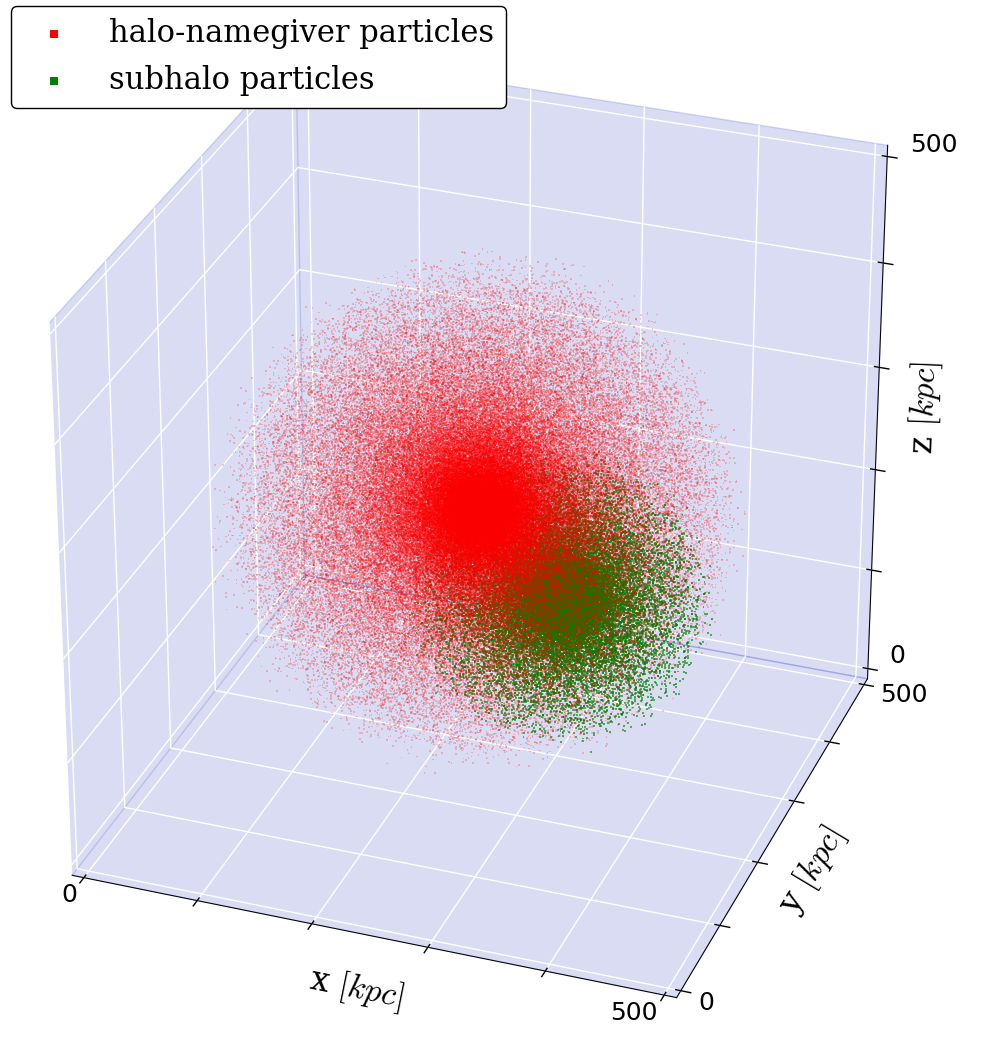
\includegraphics[height=\textwidth]{../report/images/dice-two/dice-two-original-plot.png}}%
		\caption{\footnotesize
			The initial particle distribution of the \dt\ dataset. A smaller halo (subhalo 1) made of 40'000 particles is nested within a bigger halo (halo-namegiver), which contains 200'000 particles.
		}%
		\label{fig:dice_two_origin}
		\endminipage%\hspace{.1cm}
		\hspace*{\fill}
		%
		\minipage[t]{0.497\textwidth}
		\centering
		\fbox{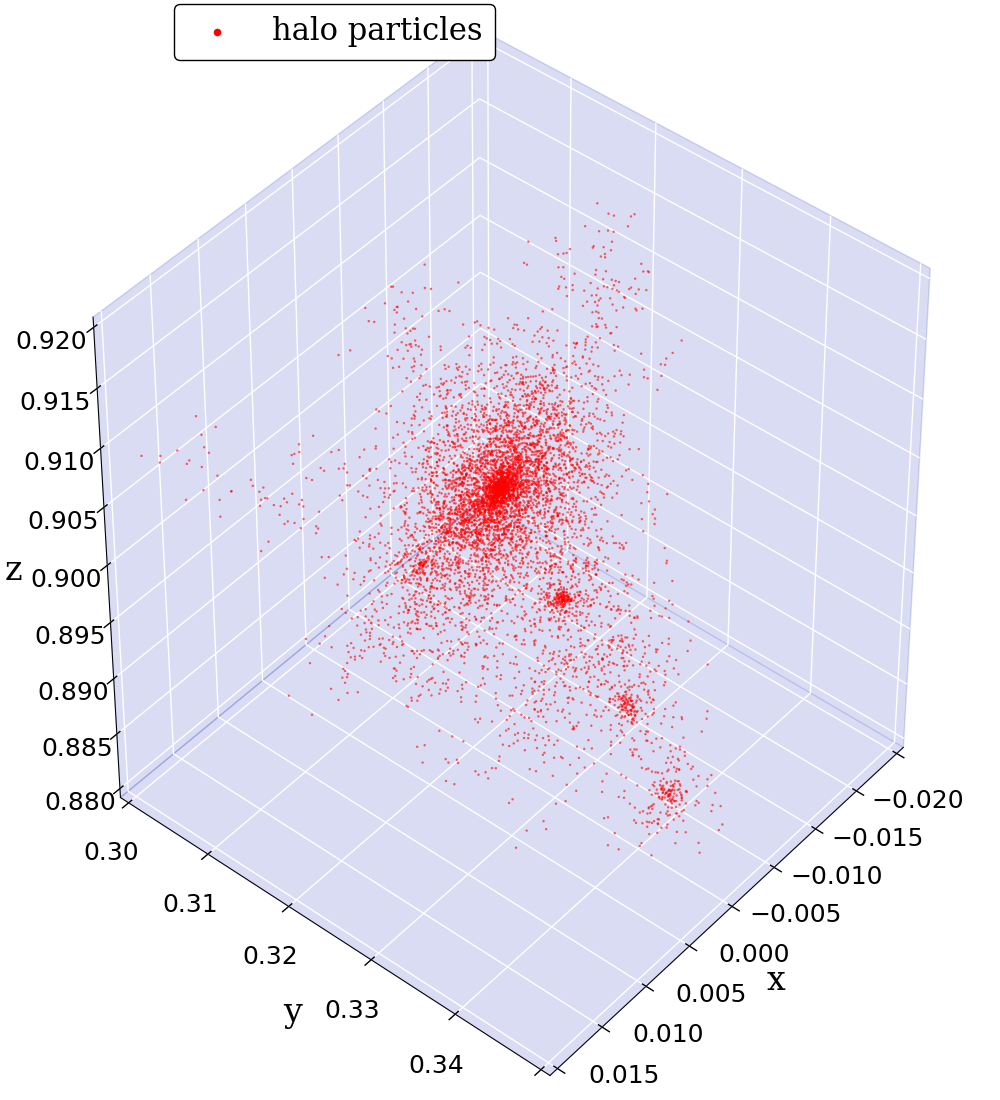
\includegraphics[height=\textwidth, keepaspectratio]{./images/cos-fullhalo-66858.png}}%
		\caption{\footnotesize
			\cosmo-dataset: A halo as identified by \phew\ of the previously shown cosmological simulation at redshift $z = 0$. 
		}%
		\label{fig:dice_sub_origin}
		\endminipage\hspace*{\fill} 
	\end{figure}
\end{frame}



%\begin{frame}
%	\frametitle{Test Cases}
%	
%	\begin{columns}
%		\column{.25\textwidth}
%		Third test case: A halo from the cosmological simulation containing  $128^3$ dark
%		matter particles at redshift $z = 0$ with $H_0 = 70.4$ and density parameters $\Omega_m = 0.272$ and $\Omega_\Lambda= 0.728$.
%		The box length corresponds to 88.8 Mpc.
%		\vfill
%		\column{.75\textwidth}
%		\begin{figure}
%			\centering
%			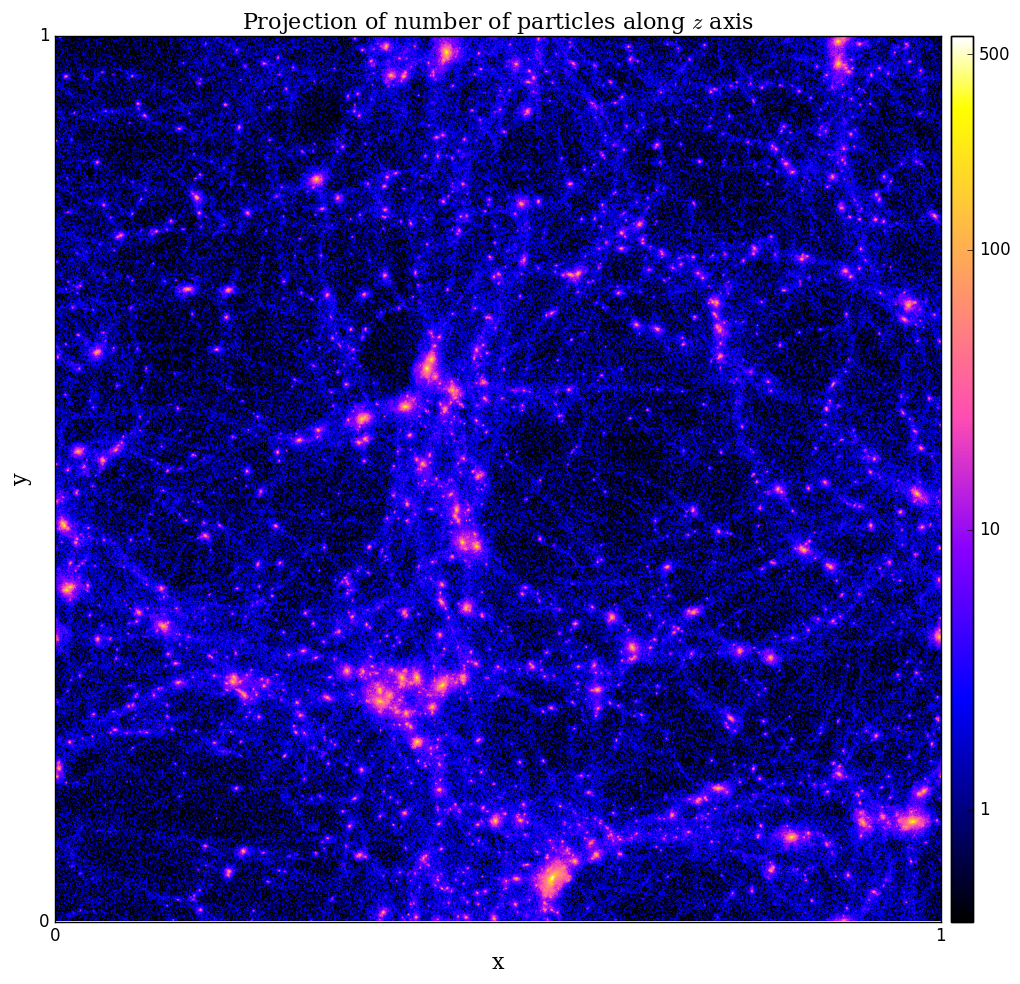
\includegraphics[width=8.2cm]{../report/images/cosmo/cos-part2map-npart.png}
%			%		\caption{
%			%		}
%		\end{figure}
%		\vfill
%	\end{columns}
%	
%\end{frame}